
\documentclass[a4paper]{article}
\usepackage[fontset=fandol]{ctex}
\usepackage{amsmath, amssymb}
\usepackage{graphicx}
\usepackage[margin=2.3cm]{geometry}
\usepackage[most]{tcolorbox}
\usepackage{listings}
\usepackage{hyperref}
\usepackage{booktabs}
\usepackage{float}
\usepackage{xcolor}

\lstset{
    basicstyle=\ttfamily\small,
    breaklines=true,
    frame=single,
    numbers=left,
    numberstyle=\tiny\color{gray}
}

\newtcolorbox{knowledgebox}[1]{
    enhanced,
    colback=blue!5!white,
    colframe=blue!70!black,
    colbacktitle=blue!70!black,
    coltitle=white,
    fonttitle=\bfseries,
    title=#1,
    sharp corners
}

\newtcolorbox{importantbox}[1]{
    enhanced,
    colback=yellow!10!white,
    colframe=yellow!70!black,
    colbacktitle=yellow!70!black,
    coltitle=black,
    fonttitle=\bfseries,
    title=#1,
    sharp corners
}

\newtcolorbox{warningbox}[1]{
    enhanced,
    colback=red!5!white,
    colframe=red!70!black,
    colbacktitle=red!70!black,
    coltitle=white,
    fonttitle=\bfseries,
    title=#1,
    sharp corners
}

\begin{document}

\begin{titlepage}
\centering
{\Large 课程讲义\par}
\vspace{1.2cm}
{\huge\bfseries Abstraction and Discovery with Large Language Model Agents\par}
\vspace{0.4cm}
{\Large CS294/194-280: Advanced Large Language Model Agents\par}
\vspace{0.4cm}
{\large Swarat Chaudhuri, The University of Texas at Austin\par}
\vspace{0.4cm}
{\large 中文教材化讲义 / Harness Build\par}
\vspace{0.8cm}
\includegraphics[width=0.84\textwidth,height=0.38\textheight,keepaspectratio]{cover.jpg}\par
\vfill
\begin{tcolorbox}[width=0.92\textwidth,colback=black!2!white,colframe=black!60,sharp corners]
\textbf{课程页}：\href{https://rdi.berkeley.edu/adv-llm-agents/sp25}{https://rdi.berkeley.edu/adv-llm-agents/sp25}\par
\textbf{录播}：\href{https://www.youtube.com/live/IHc0TEMrEdY}{https://www.youtube.com/live/IHc0TEMrEdY}\par
\textbf{Slides}：\href{https://rdi.berkeley.edu/adv-llm-agents/slides/swarat.pdf}{swarat.pdf}\par
\textbf{补充 readings}：COPRA / LaSR
\end{tcolorbox}
\end{titlepage}

\tableofcontents
\newpage

\section{本讲学习目标}

本讲把课程带到一个更高层的主题：\textbf{LLM agent 不只是求解器，还可能成为 abstraction 和 discovery 的参与者。} 读完本章后，读者应当能够：
\begin{itemize}
\item 解释 discovery agent 的四个关键能力：系统搜索、利用先验知识、从经验学习搜索策略、发明抽象概念。
\item 区分 neural-only mathematics、formal representation、autoformalization、theorem proving 与 formal verification。
\item 说明 COPRA 为什么是一个真正的 theorem-proving agent，而不只是把 GPT-4 直接套到 proof assistant 上。
\item 理解 compiler verification 例子中 definitions、theorem statement、lemma invention 与 automated proving 的关系。
\item 解释 symbolic regression 在 scientific discovery 中的作用，以及 LaSR 为什么要学习 concept library。
\item 把概念抽象（abstraction）看成搜索空间重构机制，而不是装饰性的术语生成。
\end{itemize}

\section{从课程回顾到 discovery 视角}

\subsection{为什么这一讲不是上一讲的简单延续}

前一讲主要讨论 theorem proving 内部的系统设计：thought、sketch、premise selection、long-context formalization。这一讲虽然继续讨论数学与证明，但视角更广。Swarat Chaudhuri 一开始先回顾整门课已经展示过的 LLM 用法，然后指出：如果只把 LLM 当作 ``答题机器''，我们最多是在已有问题上求更好答案；若把它当成 \textbf{scientific and mathematical discovery} 的工具，我们关心的就变成了如何提出 hypothesis、发明抽象、组织 search，以及从历史尝试中学习更好的探索方式。

\subsection{discovery agent 的四个关键能力}

\begin{figure}[H]
\centering
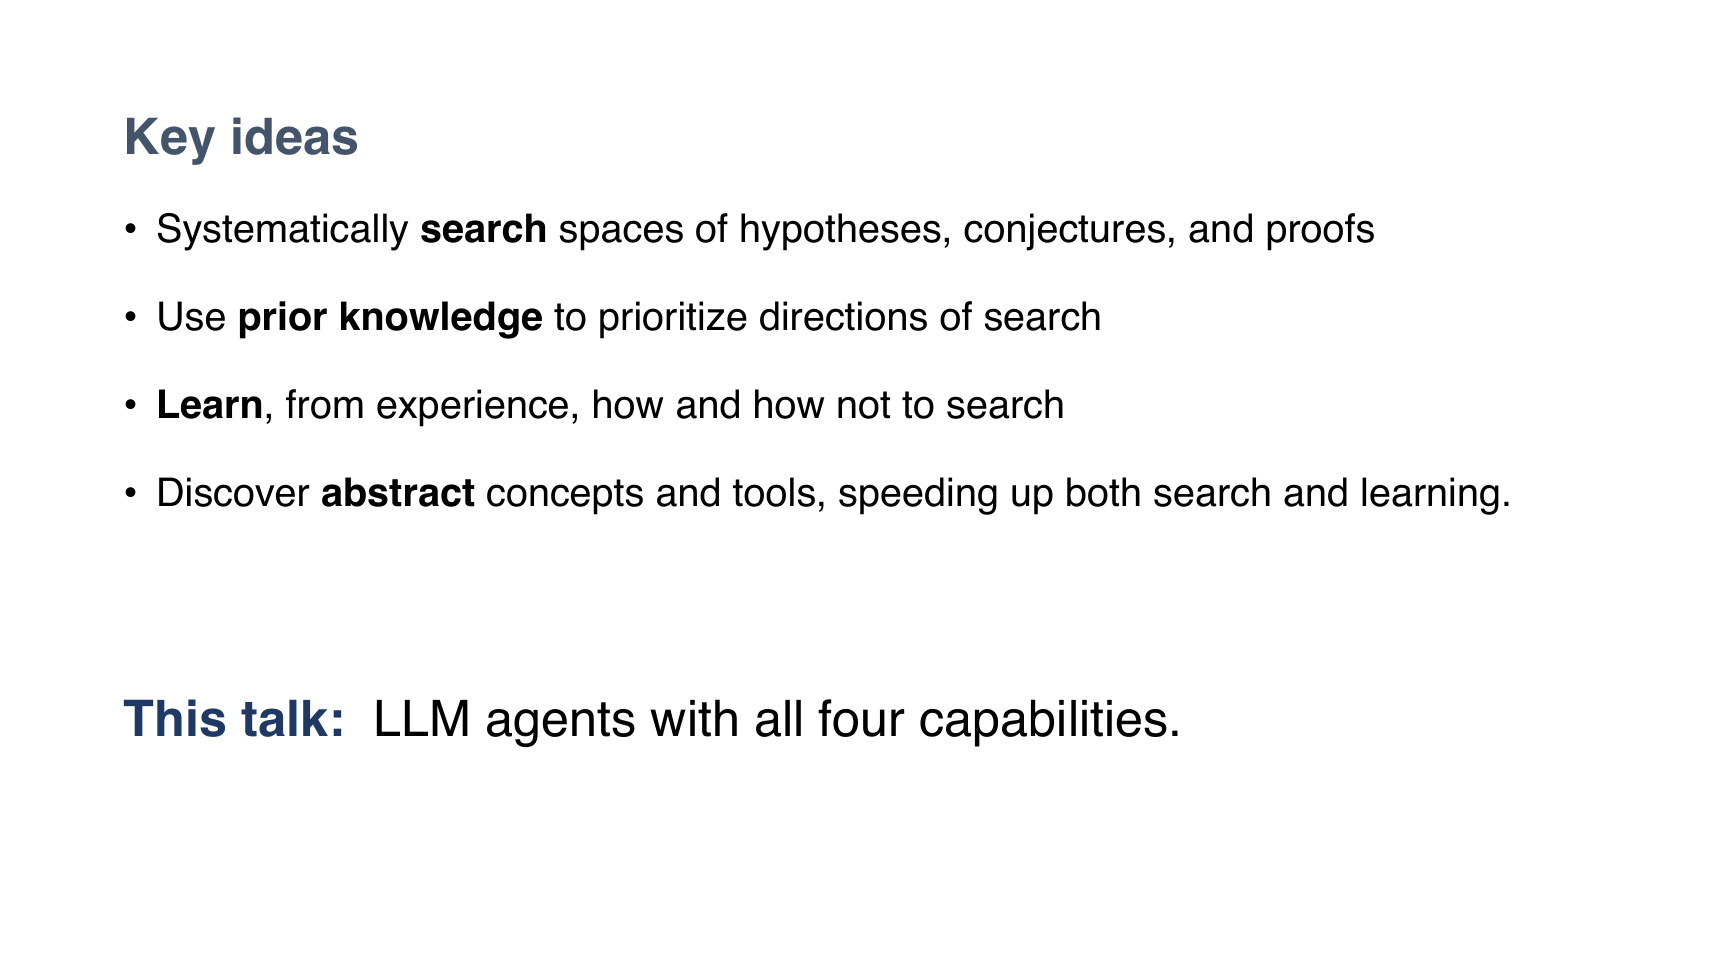
\includegraphics[width=0.82\textwidth]{figures/lec11_fig_001.png}
\caption{本讲的四个 key ideas：search、prior knowledge、learning from experience、discovered abstractions。}
\end{figure}

slides 第 4 页给出的四个能力是本讲的主轴：
\begin{enumerate}
\item \textbf{Systematically search spaces of hypotheses, conjectures, and proofs}：不是只对单个答案打分，而是显式搜索可能的假设、猜想和证明。
\item \textbf{Use prior knowledge to prioritize directions of search}：利用已有知识偏向更有希望的区域。
\item \textbf{Learn, from experience, how and how not to search}：从成功与失败中更新搜索策略。
\item \textbf{Discover abstract concepts and tools}：不是只在既有 primitive 上搜索，而是发明新的概念来重构搜索空间。
\end{enumerate}

\begin{knowledgebox}{这四点为什么重要}
如果只做前两点，系统更像一个强检索器；如果加入第三点，它开始像能自适应的 agent；如果加入第四点，它就不再只是在固定语言里搜索，而是在 \emph{改变} 语言本身。
\end{knowledgebox}

\subsection{neural-only approach 的局限}

讲座随后用数学题推理示例和 OpenAI o1 的例子说明，强大的 neural-only model 的确能做出惊人的数学推理。但 Swarat 紧接着给出两个硬约束：\textbf{数据稀缺（data scarcity）}和\textbf{缺乏可验证性（lack of verifiability）}。高质量 proof traces、严格 reward functions 在 research-level mathematics 中并不充足；同时，自然语言 reasoning 极难完全验证，而科学和验证任务往往最怕遗漏 edge case。于是，lecture 的方向不是否定 neural model，而是问：\textbf{如何把 formal representation、environment feedback 与 abstraction 结合进来。}

\section{formal representations：把问题接入可验证环境}

\subsection{从 informal problem 到 formal proof}

\begin{figure}[H]
\centering
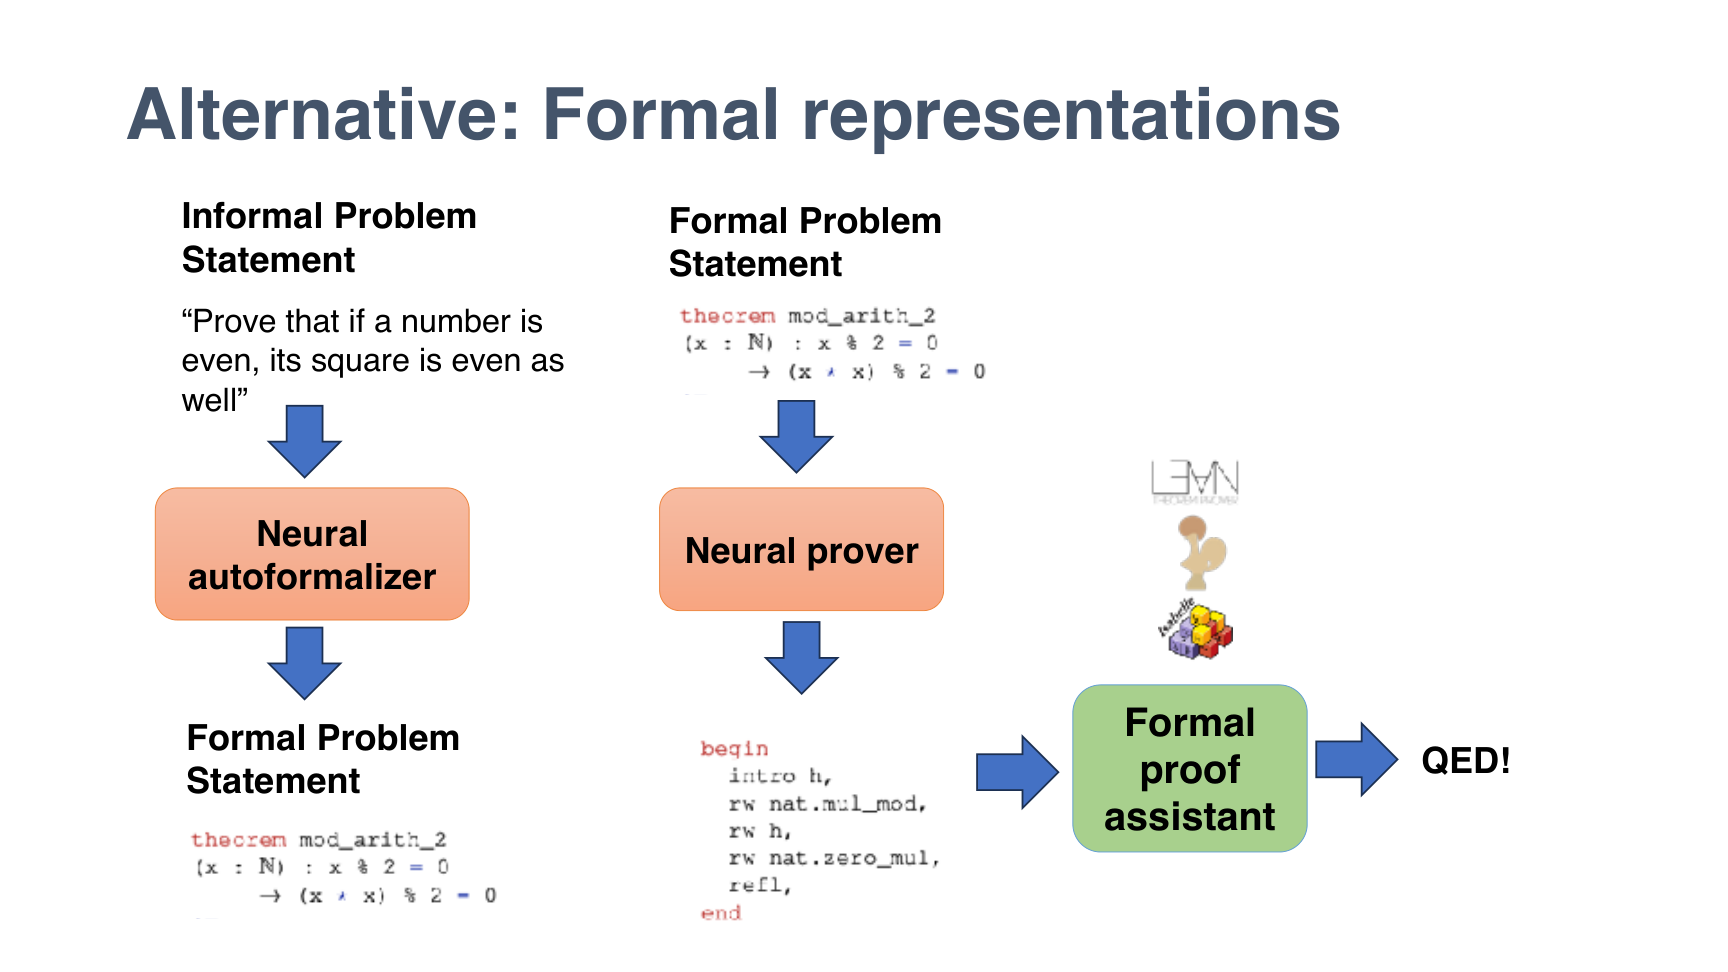
\includegraphics[width=0.80\textwidth]{figures/lec11_fig_002.png}
\caption{formal representation pipeline：informal problem 先转成 formal statement，再进入 proof assistant 与 neural prover。}
\end{figure}

Slides 9--12 把一个简单数学命题放进 formal pipeline：先把自然语言问题写成正式 theorem statement，再由 proof assistant 或 neural prover 搜索证明。用一个简洁的形式可以写成：
\[
x_I \xrightarrow{\mathcal{A}} x_F \xrightarrow{\mathcal{P}} \tau
\]
其中 $x_I$ 是 informal problem statement，$\mathcal{A}$ 表示 autoformalizer 或 formal representation builder，$x_F$ 是 formal theorem statement，$\mathcal{P}$ 表示 prover，而 $\tau$ 则是最终 formal proof trajectory。

\paragraph{符号解释}
\begin{itemize}
\item $x_I$：人类自然语言或半结构化形式下的问题。
\item $\mathcal{A}$：把自然语言问题翻译成 proof assistant 能理解的规范表示。
\item $x_F$：可检验的 theorem statement。
\item $\mathcal{P}$：在 formal system 中进行证明搜索的过程。
\item $\tau$：最终被 proof assistant 接受的证明轨迹。
\end{itemize}

\subsection{必须区分的几个概念}

这部分最容易混淆，必须严格拆开：
\begin{itemize}
\item \textbf{Autoformalization}：从自然语言题目或数学文本得到 formal statement。
\item \textbf{Theorem proving}：在 formal statement 给定的情况下，搜索 proof。
\item \textbf{Verification}：检查 proof 是否满足 formal system 规则。
\item \textbf{Informal reasoning}：帮助提出 subgoal、proof sketch 或直觉，但本身不构成 machine-checked certificate。
\end{itemize}

这一讲刻意把这几层并列，是为了说明 discovery agent 不是只做其中一层，而是可能把这些层串起来。上一讲强调 theorem proving 的内部系统工程；本讲强调如何把 proving、verification 与更高层 abstraction 绑定到一起。

\section{COPRA：formal theorem-proving agent}

\subsection{为什么 COPRA 是 agent，不是 prompt trick}

\begin{figure}[H]
\centering
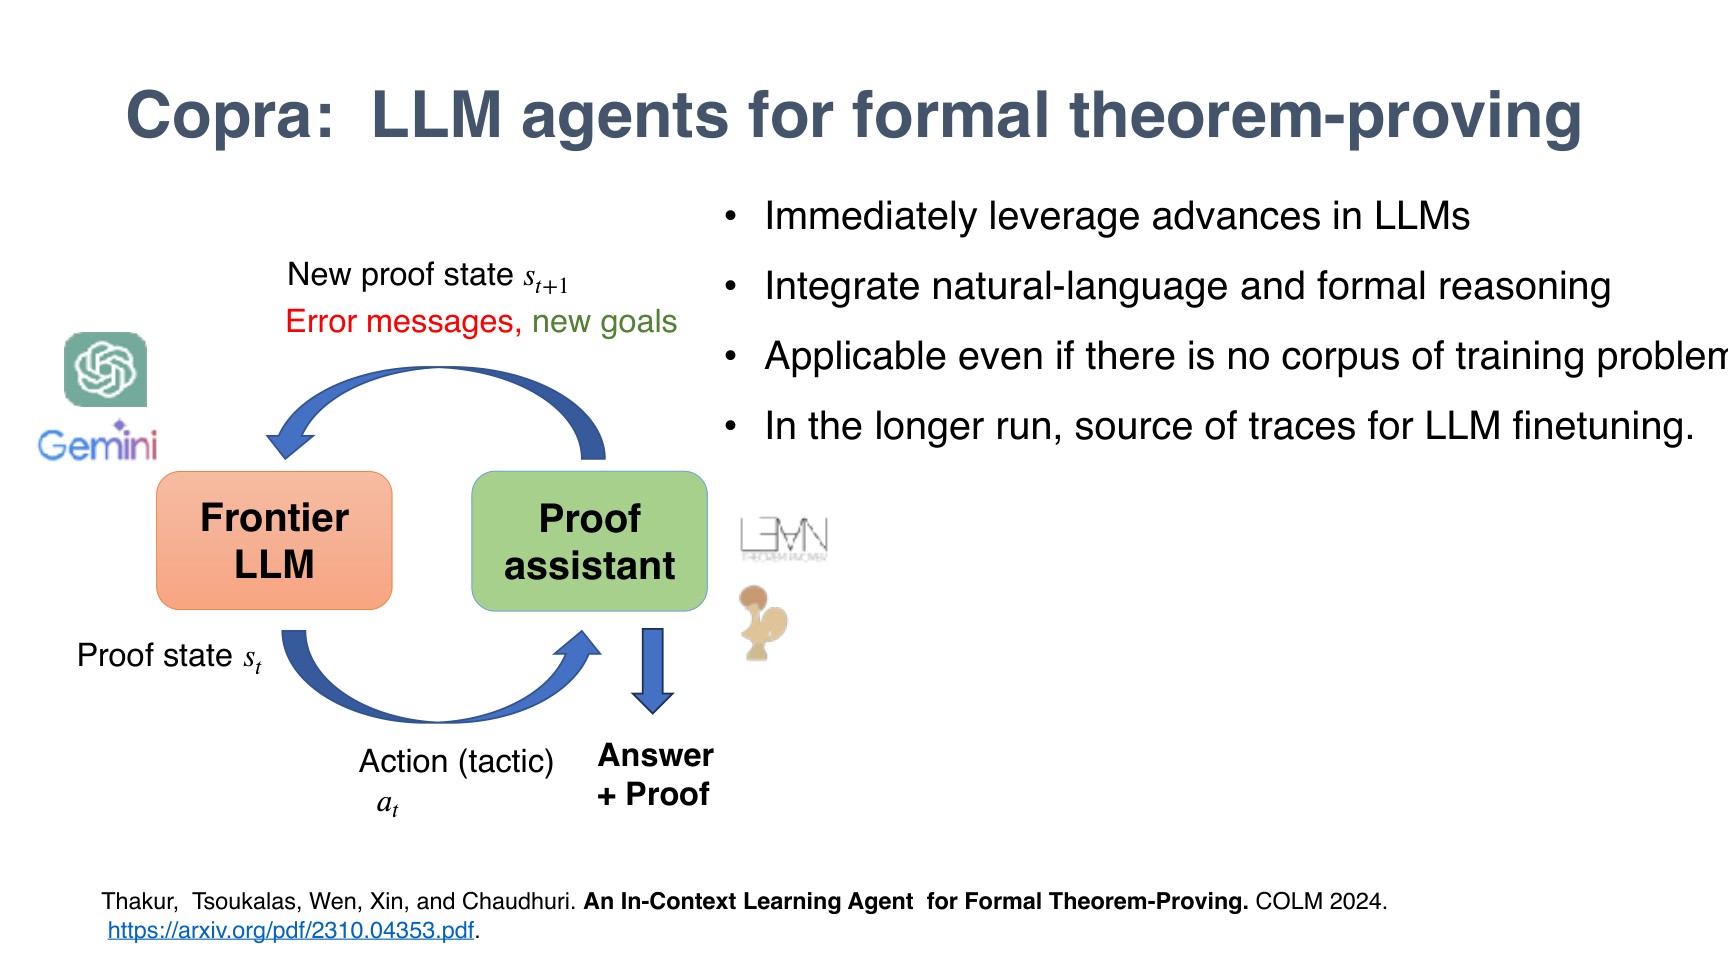
\includegraphics[width=0.82\textwidth]{figures/lec11_fig_003.png}
\caption{COPRA 作为 theorem-proving agent：frontier LLM、proof assistant、proof state 与错误反馈形成闭环。}
\end{figure}

COPRA（\emph{An In-Context Learning Agent for Formal Theorem-Proving}）的核心贡献在于：它不依赖大量 environment-specific finetuning，而是让强 LLM 在一个 \textbf{stateful backtracking search} 里不断读取 proof state、提出 tactic、执行 tactic、接收错误与新 goals，然后再把这些信息写回 prompt。这里的 agent 性主要体现在三个方面。

第一，它和 proof environment 持续交互，而不是一次性生成整段 proof。第二，它维护 search history，并在失败后回溯。第三，它把 lemma database 和 informal hints 当作外部资源纳入决策。也就是说，它具备 environment、memory、tool use 和 feedback 这几个 agent 组件。

\subsection{COPRA 的 loop}

\begin{figure}[H]
\centering
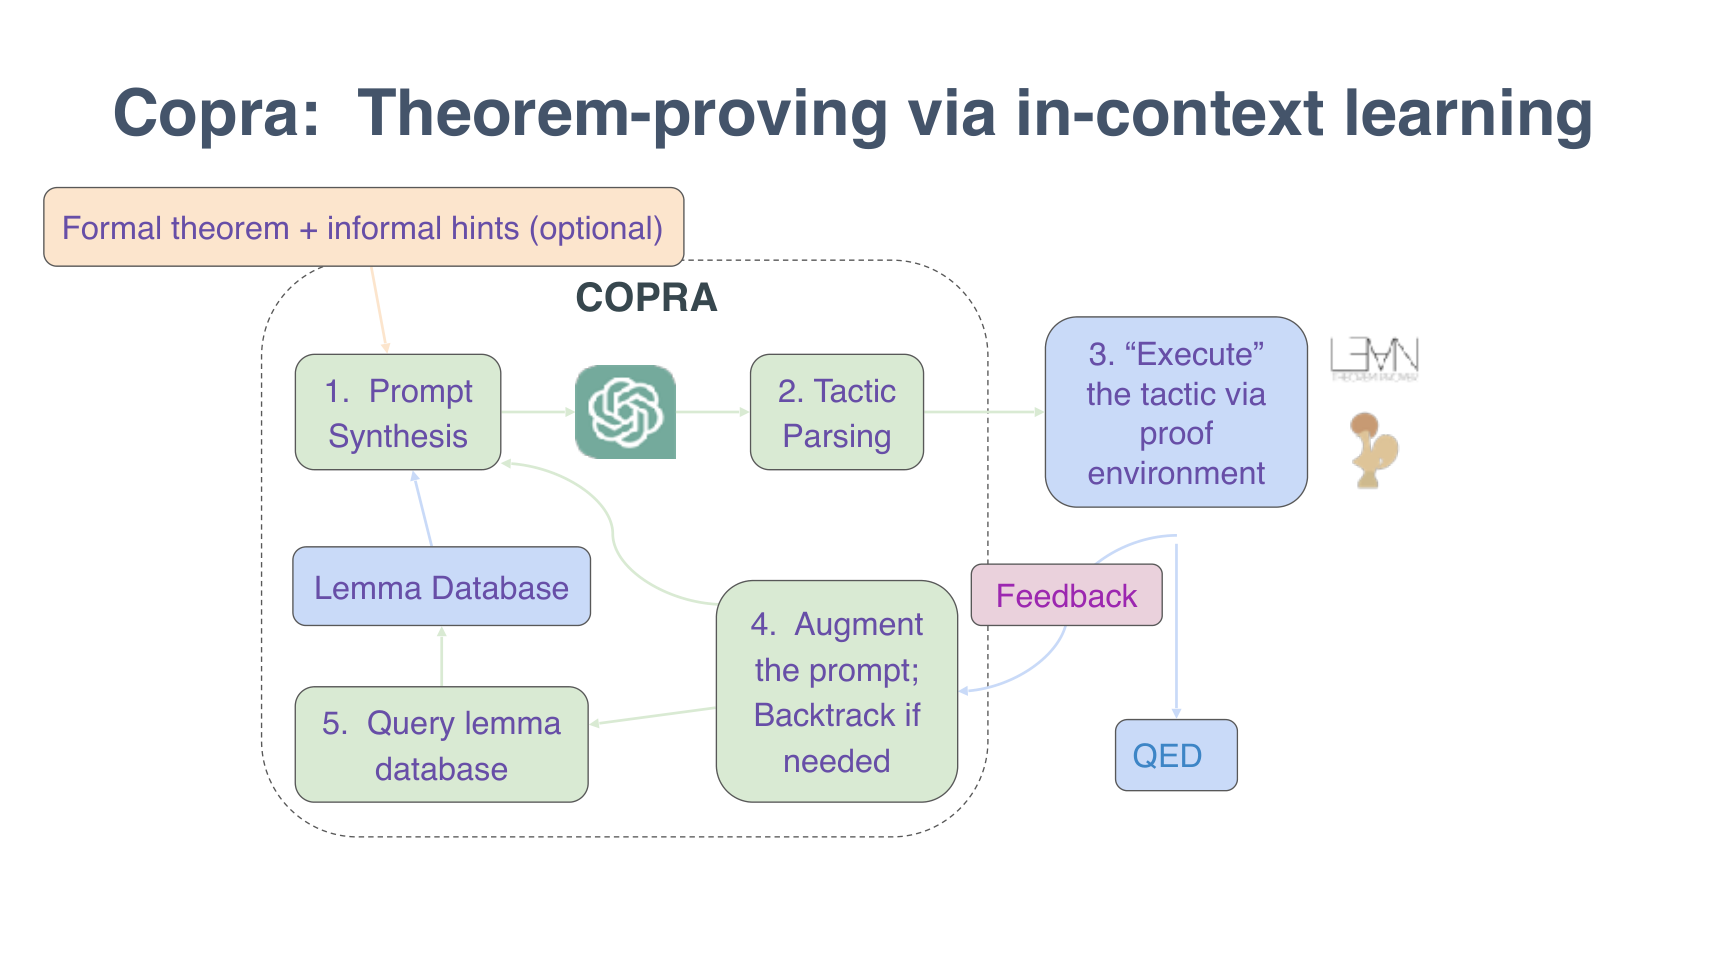
\includegraphics[width=0.80\textwidth]{figures/lec11_fig_004.png}
\caption{COPRA 的 in-context proving loop：prompt synthesis、action parsing、proof execution、feedback augmentation 与 lemma retrieval。}
\end{figure}

这部分可以写成一个环境驱动的 search objective：
\[
\tau^{\star} = \arg\max_{\tau \in \mathcal{S}(s_0)} \sum_{t=0}^{T} r_{\mathrm{env}}(s_t, a_t)
\]
其中 $\tau$ 是 proof trajectory，$\mathcal{S}(s_0)$ 是从初始 state $s_0$ 出发的可探索轨迹集合，$r_{\mathrm{env}}$ 是 proof environment 返回的反馈信号，$s_t$ 是当前 proof state，$a_t$ 是 tactic action。

\begin{lstlisting}
Initialize proof state s0 and prompt context
Query the LLM for a tactic proposal
Parse and execute the tactic in the proof environment
Append new goals, errors, and lemmas to the prompt
Backtrack or continue until QED or budget exhaustion
\end{lstlisting}

这一算法的本质，是把 proof assistant 变成 verifier + environment。和一般自然语言 agent 相比，它的反馈更严格，因为动作一旦非法就会立刻报错；但 action space 也更苛刻，因为 tactic 不只是语义上大致正确，而必须语法与类型上都合法。

\subsection{为什么 lecture 要讲 natural-language 与 formal reasoning 的结合}

Slides 20--24 特别展示，COPRA 不必把所有推理都压缩成 formal tactic。相反，它可以先让模型用自然语言产生高层 decomposition，例如把 theorem 拆成几个 sub-goals，再让 formal prover 分别解决。这与上一讲的 Draft, Sketch, Prove 有明显呼应，但侧重点不同：DSP 更强调用 sketch 引导 low-level prover，而 COPRA 更强调在 proving loop 内动态地使用 informal hints、lemma retrieval 和 history。

\begin{importantbox}{精确区分}
这里的 informal reasoning 是 search scaffold，不是 proof certificate。最终 correctness 仍由 proof assistant 保证，而不是由自然语言解释保证。
\end{importantbox}

\section{formal verification：从数学证明走向软件正确性}

\subsection{formal verification 的问题结构}

\begin{figure}[H]
\centering
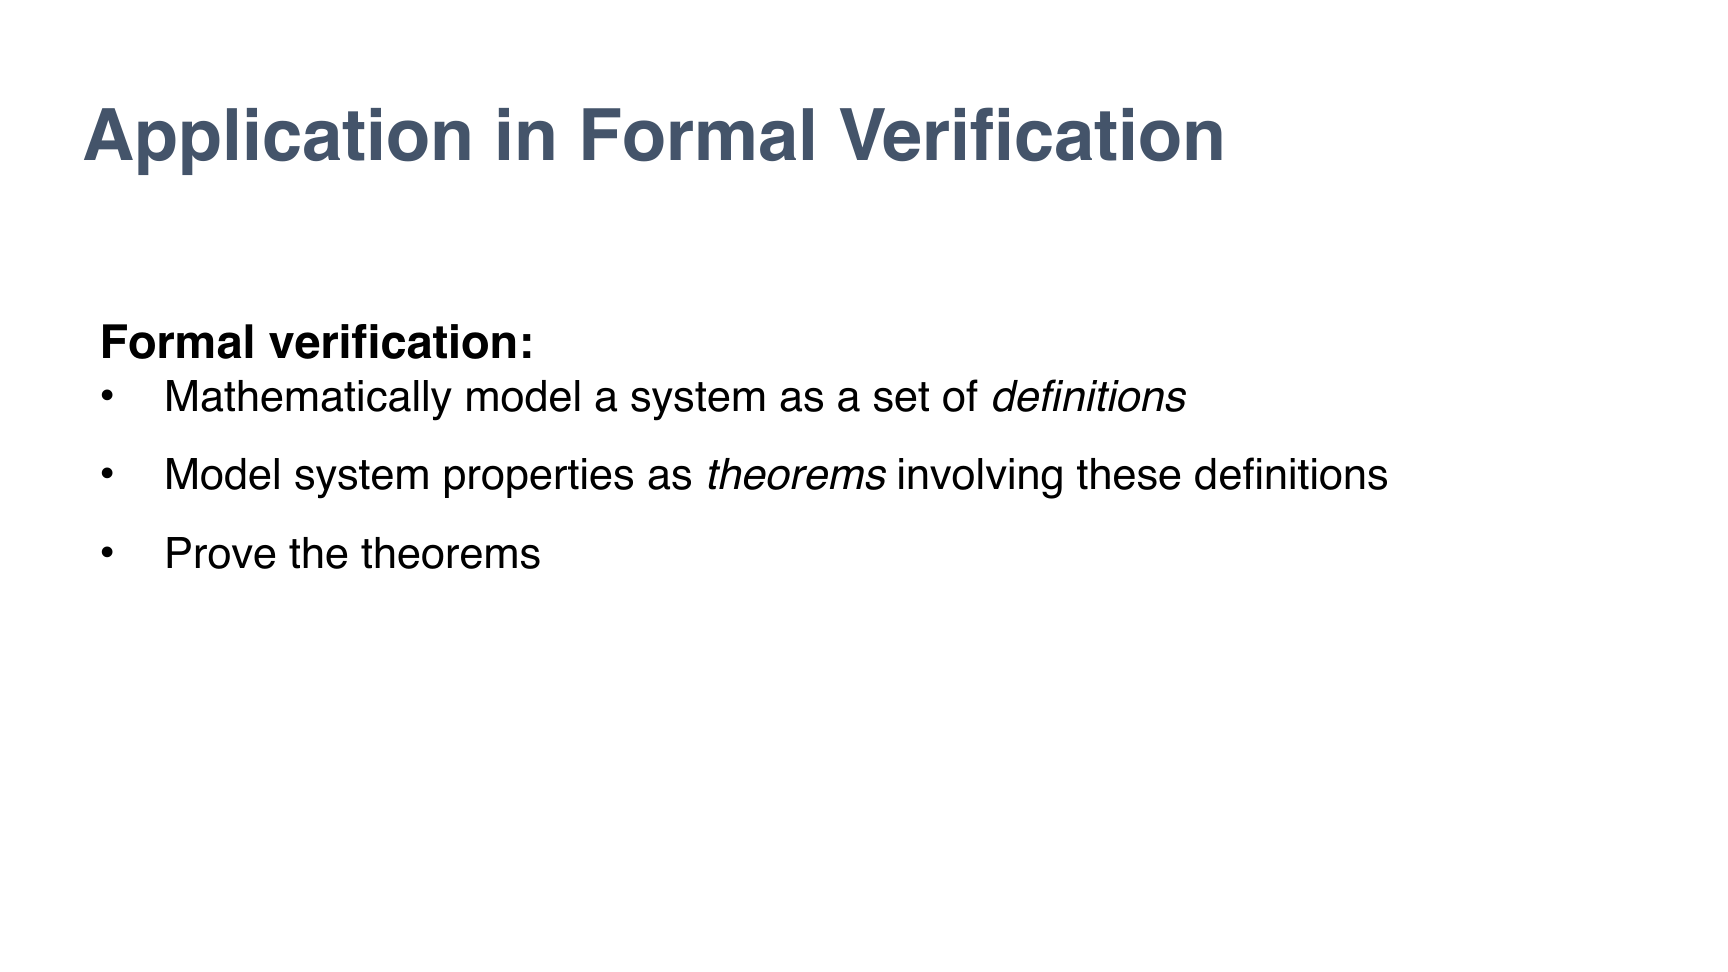
\includegraphics[width=0.82\textwidth]{figures/lec11_fig_005.png}
\caption{formal verification 的基本结构：定义系统、陈述性质、再把性质写成 theorem 来证明。}
\end{figure}

讲座在这里故意从纯数学 theorem 转向 compiler verification。原因是：formal verification 更接近实际 agent 应用，它要求系统先写出语言语法、语义、编译器，再证明 correctness theorem。也就是说，agent 不只是 ``解题''，而是在一个更大的 specification + implementation + proof workflow 里工作。

\subsection{compiler correctness 例子}

slides 26--39 逐步构造 source language、target language、compile 函数和 correctness theorem，最后要求系统证明：

\begin{figure}[H]
\centering
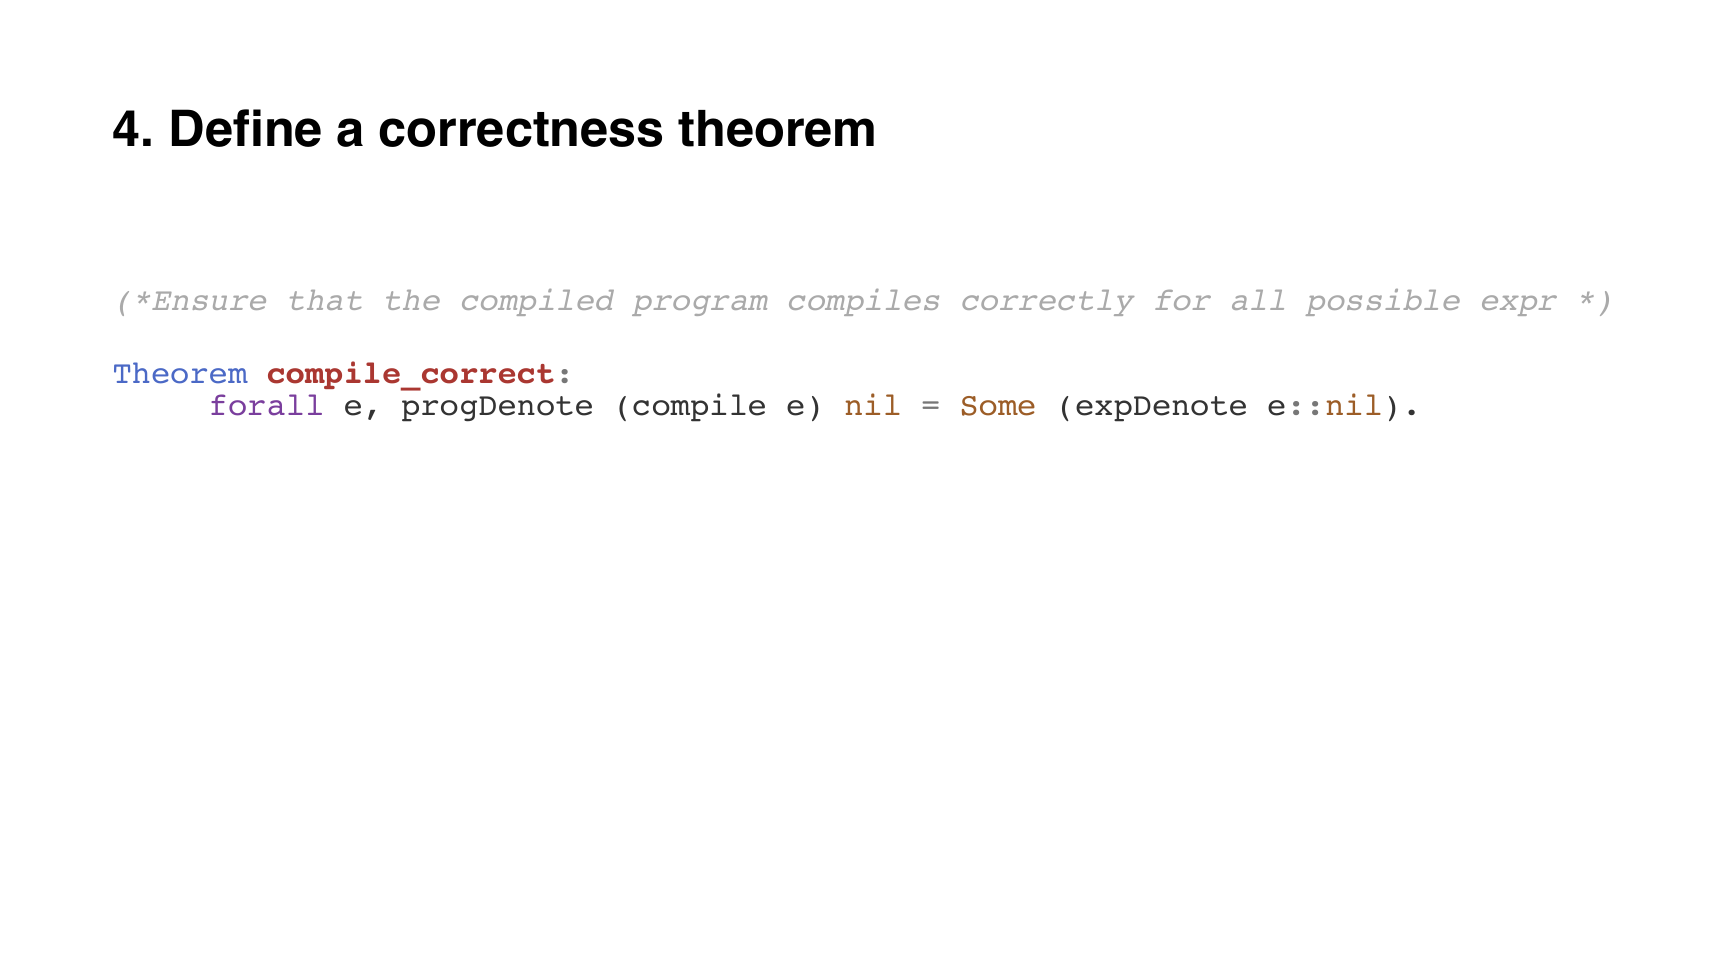
\includegraphics[width=0.82\textwidth]{figures/lec11_fig_006.png}
\caption{compiler correctness theorem：lecture 用它说明 theorem-proving agent 如何服务 formal verification。}
\end{figure}

在 lecture 里，证明不只是把现成 theorem 扔给 prover，而是包含 lemma invention、subgoal decomposition 和 tactic 执行。换言之，verification agent 至少要理解：
\begin{itemize}
\item 问题的 \textbf{语义对象} 是什么；
\item correctness theorem 的输入输出如何定义；
\item 哪些中间 lemma 需要先被发明出来；
\item proof assistant 的错误信息如何反向指导下一步搜索。
\end{itemize}

\begin{lstlisting}
Define source language semantics
Define target machine semantics
Implement compile
State compile_correct theorem
Use the prover to derive helper lemmas and prove compile_correct
\end{lstlisting}

这也是本讲中 verification 与 theorem proving 的准确关系：verification 任务往往通过 theorem proving 来完成，但 verification 还额外要求 specification 建模与边界条件覆盖。

\section{从数学 discovery 到科学 discovery}

\subsection{scientific discovery lifecycle}

\begin{figure}[H]
\centering
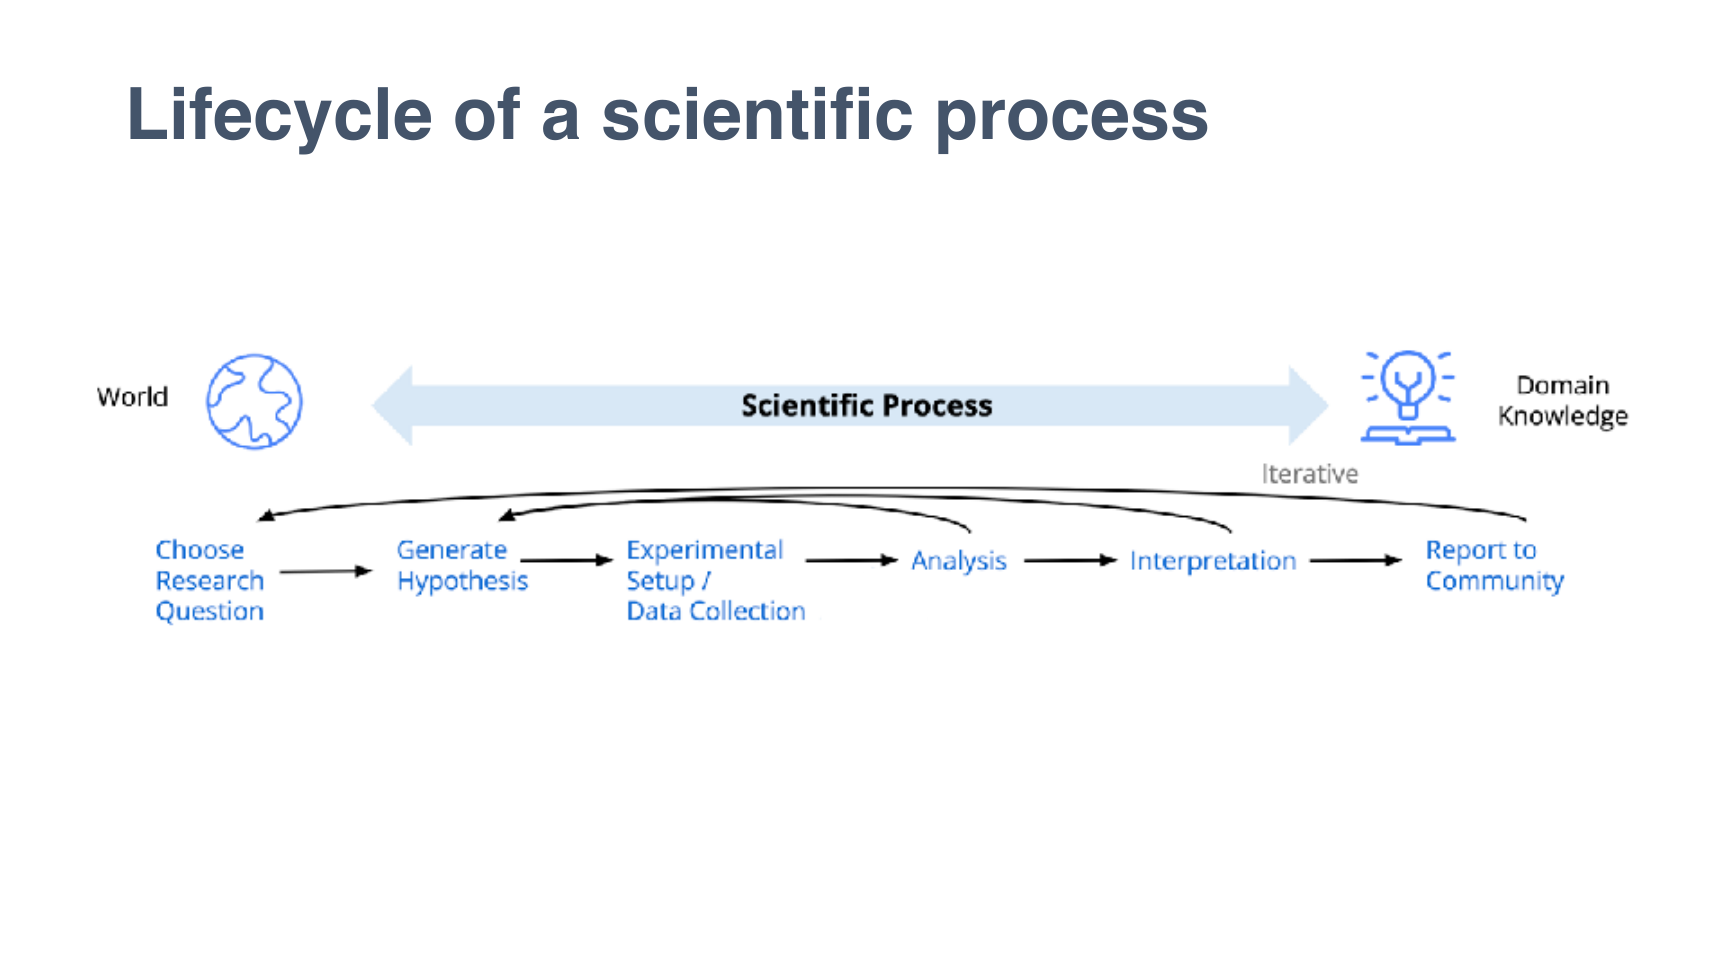
\includegraphics[width=0.82\textwidth]{figures/lec11_fig_007.png}
\caption{scientific discovery lifecycle：从数据、假设、建模到实验设计的闭环。}
\end{figure}

下半场 lecture 把视角扩展到 empirical science。slides 第 46 页给出 scientific process 的生命周期：收集数据、提出 hypothesis、建模 theorizing、设计或运行实验、再用结果反哺 hypothesis。这里与 theorem proving 的共同点是都需要 search；不同点是，科学 discovery 的 verifier 往往更弱、更贵，甚至只能由实验近似提供。

\subsection{symbolic regression 的问题形式}

在 symbolic regression 中，我们希望从数据中找出一个紧凑、可解释的程序化表达式。这可以写成：
\[
f^{\star} = \arg\min_{f \in \mathcal{H}(L)} \mathcal{L}(f; D) + \lambda \Omega(f)
\]
其中 $f$ 是候选表达式，$\mathcal{H}(L)$ 是由 concept library $L$ 支持的 hypothesis space，$D$ 是数据，$\mathcal{L}$ 是拟合损失，$\Omega$ 是复杂度正则项，$\lambda$ 控制拟合精度和表达式复杂度的权衡。

\paragraph{直觉}
如果没有 concept library，系统只能在非常原始的符号和运算符上盲搜；一旦有抽象概念，搜索就可以在更高层空间里进行。例如 ``正弦趋势''、``平方反比'' 这类概念会让 mutation 和 crossover 更像人在做物理建模时的猜想。

\section{LaSR：用 concept library 改写搜索空间}

\subsection{LaSR 的核心思想}

\begin{figure}[H]
\centering
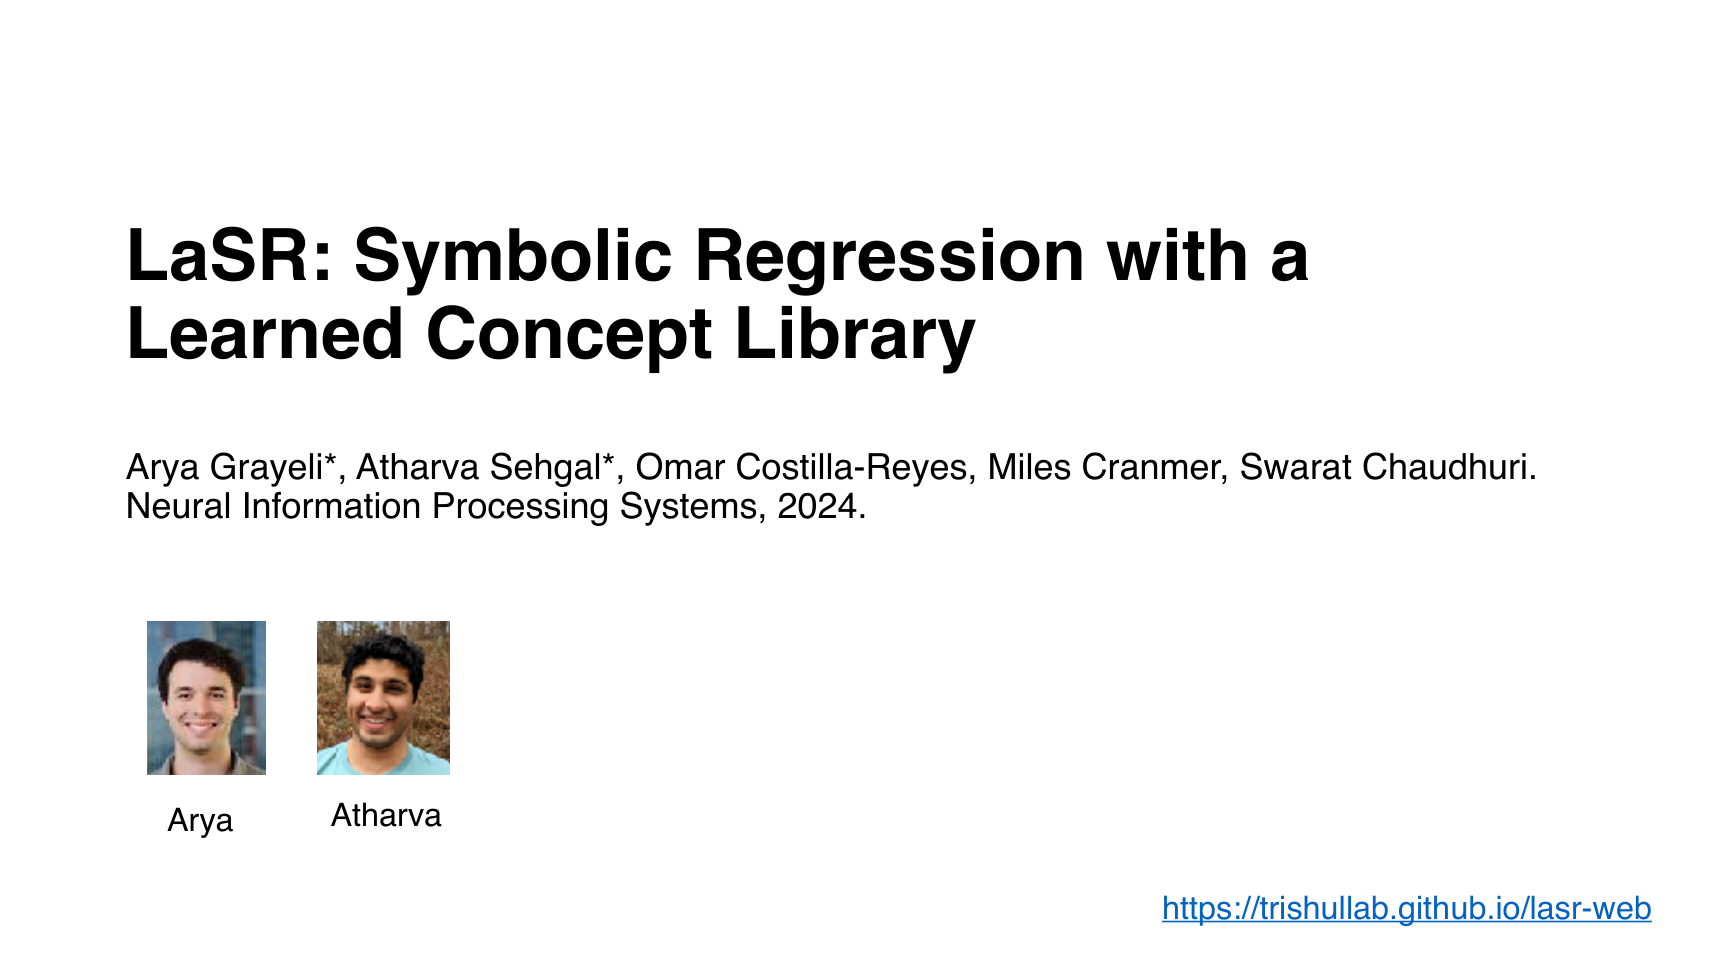
\includegraphics[width=0.80\textwidth]{figures/lec11_fig_008.png}
\caption{LaSR 的目标：在 symbolic regression 中学习和演化抽象 concept library。}
\end{figure}

LaSR（\emph{Symbolic Regression with a Learned Concept Library}）的关键，不是让 LLM 直接吐一个公式，而是把高质量 hypotheses 中反复出现的结构抽象成 concepts，再用这些 concepts 指导后续搜索。这样，LLM 的作用不是替代所有 evolutionary operator，而是向搜索器注入 \textbf{更有意义的 search basis}。

\subsection{concept abstraction 与 concept evolution}

\begin{figure}[H]
\centering
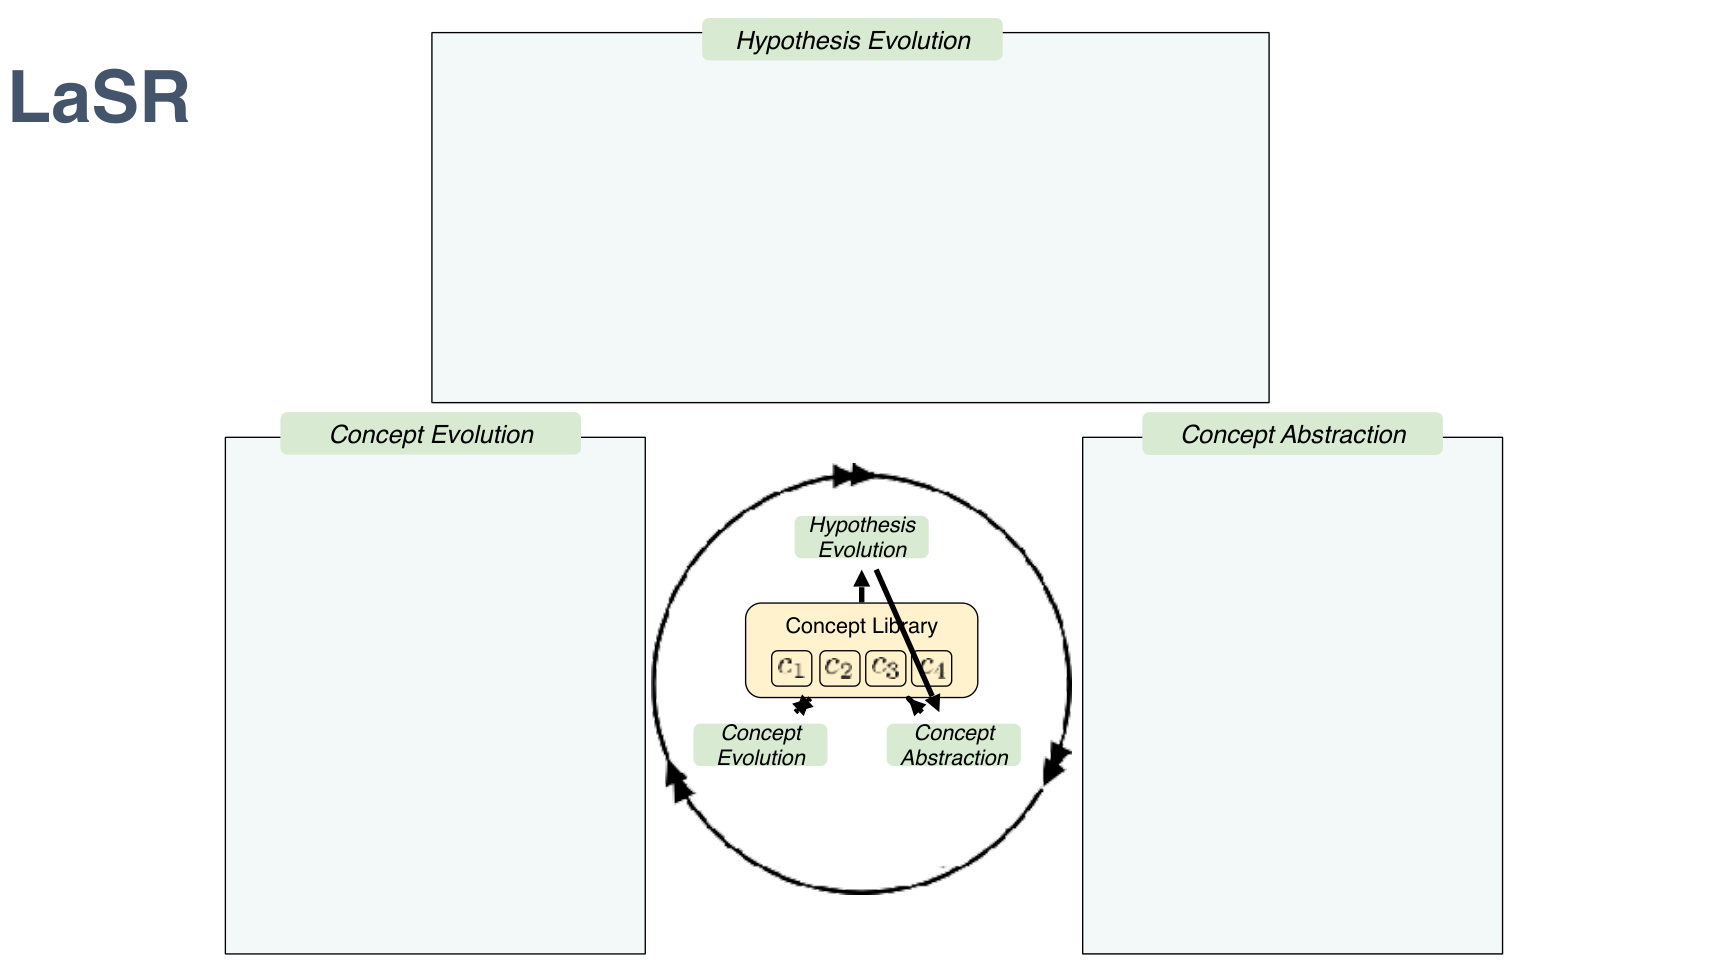
\includegraphics[width=0.78\textwidth]{figures/lec11_fig_009.png}
\caption{LaSR 的循环：hypothesis evolution、concept abstraction 与 concept evolution 相互促进。}
\end{figure}

LaSR 的迭代关系可以写成：
\[
L_{t+1} = \operatorname{Update}(L_t, H_t, D)
\]
这里 $L_t$ 是第 $t$ 轮 concept library，$H_t$ 是当前轮发现的高质量 hypotheses，$D$ 是数据或反馈，$L_{t+1}$ 是更新后的概念库。直觉上，系统先在当前 library 支持下生成 hypotheses，再从这些 hypotheses 中抽象出新的 concepts，接着用新 concepts 继续扩大下一轮搜索能力。

\begin{lstlisting}
Initialize hypothesis population H and concept library L
Fit and rank candidate equations on data
Abstract recurring symbolic concepts from top hypotheses
Query the LLM for concept-guided mutations and crossovers
Update H and L, then repeat
\end{lstlisting}

这个过程说明 abstraction 的真正价值：\textbf{它把成功经验沉淀成新 primitive，从而改变未来搜索的 geometry。} 这和 theorem proving 里发明 reusable lemma、proof sketch 或 retrieval hint 非常相似。

\subsection{为什么 concept library 能加速 discovery}

\begin{figure}[H]
\centering
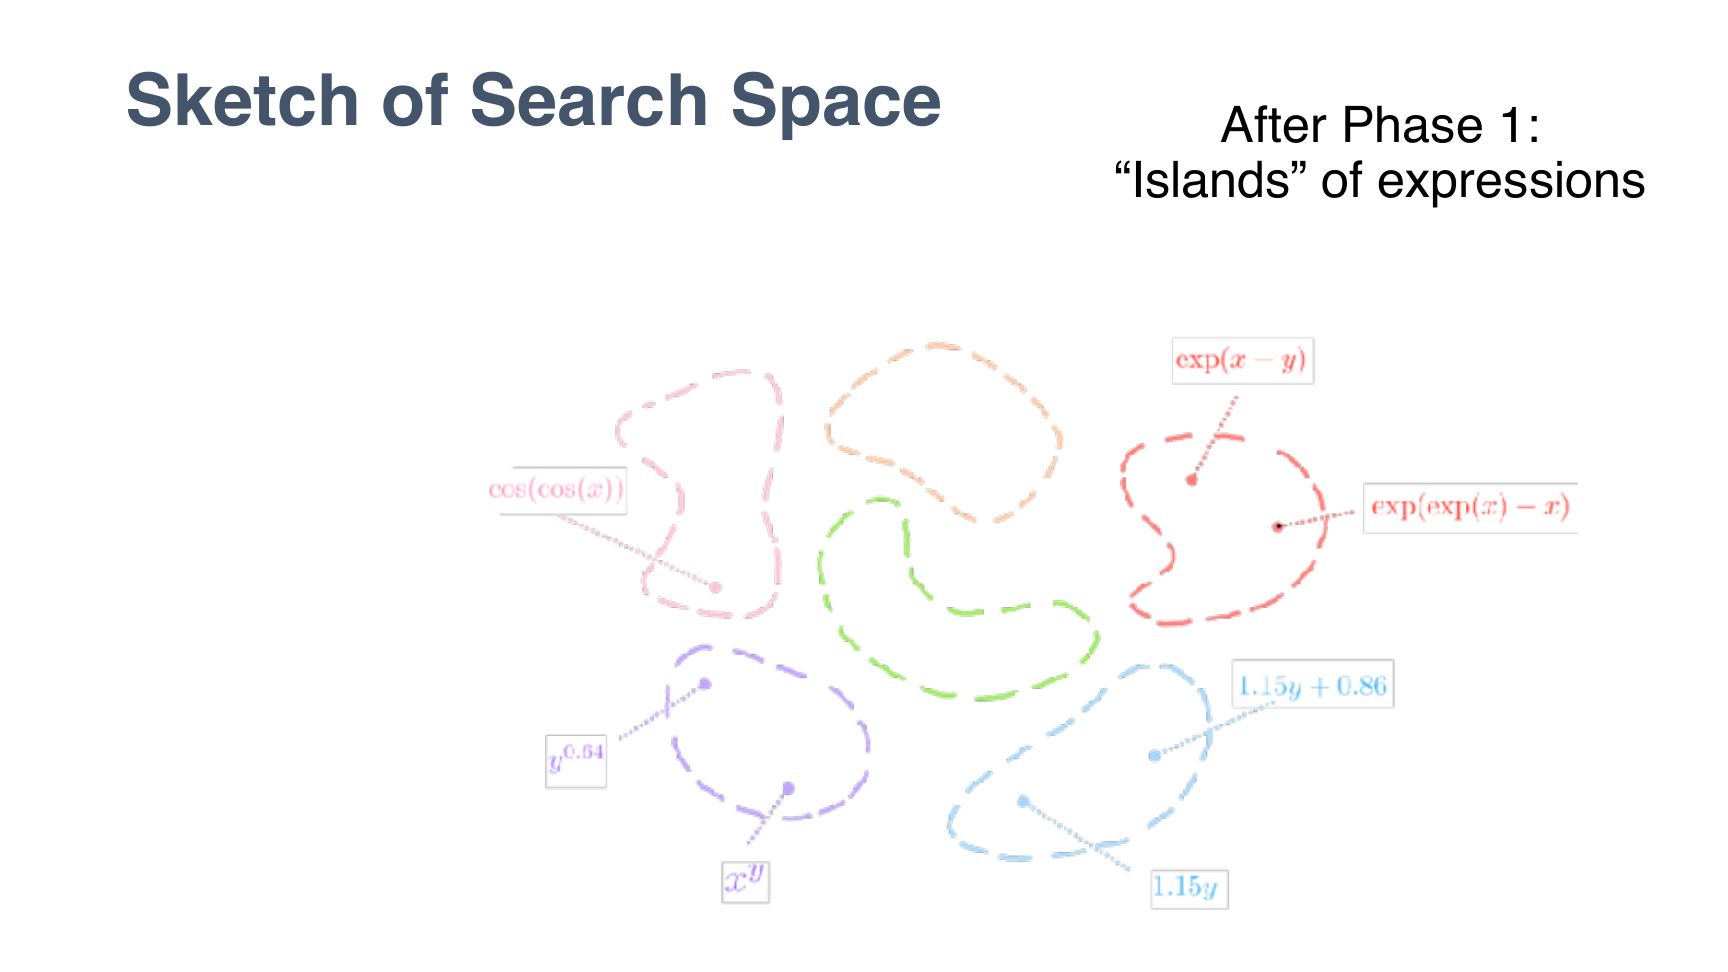
\includegraphics[width=0.80\textwidth]{figures/lec11_fig_010.png}
\caption{concept library 把搜索空间组织成更可探索的 ``islands''，从而提高搜索效率。}
\end{figure}

slides 中 ``islands of expressions'' 的图非常关键。它表明，概念库的作用不是简单地给模型多几个自然语言标签，而是把原本杂乱、巨大、局部平滑性很差的表达式空间组织成一些更容易跨越和局部搜索的区域。于是 mutation 不再只是随机换符号，而是能沿着 ``这一类函数家族'' 的方向搜索。

\subsection{结果与边界条件}

LaSR 在 Feynman equations 和 synthetic tasks 上优于多种 baseline，还能在较小本地模型的帮助下继续获益。这说明 abstraction 的收益不只是 ``大模型更聪明''，而是 \textbf{好的概念性偏置本身能改善搜索算法。} 但 lecture 也隐含指出了局限：concept quality 怎么验证？自然语言概念是不是总能对应稳定的程序结构？这些问题还远未解决。

\section{从 scaling law 到视觉概念库}

\subsection{LaSR 发现 scaling laws}

\begin{figure}[H]
\centering
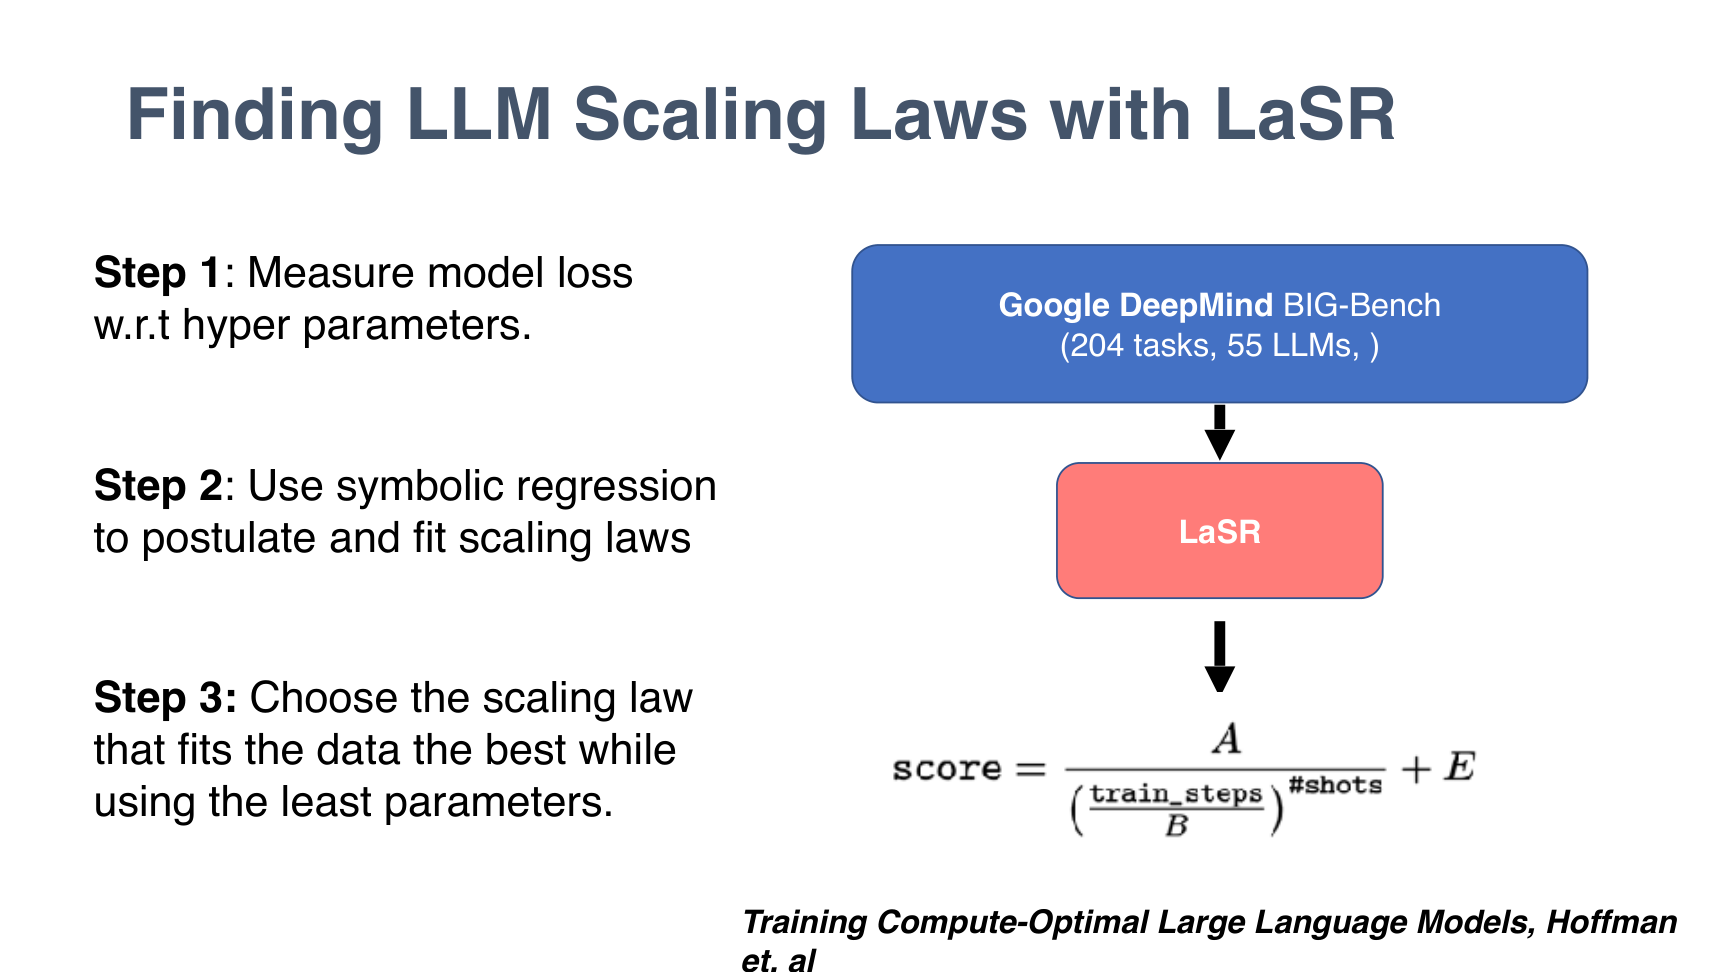
\includegraphics[width=0.82\textwidth]{figures/lec11_fig_011.png}
\caption{LaSR 在 scaling law discovery 上的使用：从实验数据中归纳紧凑可解释的 scaling 关系。}
\end{figure}

lecture 用 LLM scaling law discovery 这个例子说明：concept-guided symbolic regression 并不局限于物理公式恢复，它也可以用于从实验数据中发现简洁的经验规律。这一点特别重要，因为它表明 abstraction agent 不一定直接操作 theorem 或 proof，它也可以在 empirical modeling 中做 ``提出可解释规律'' 的工作。

\subsection{visual concept library}

\begin{figure}[H]
\centering
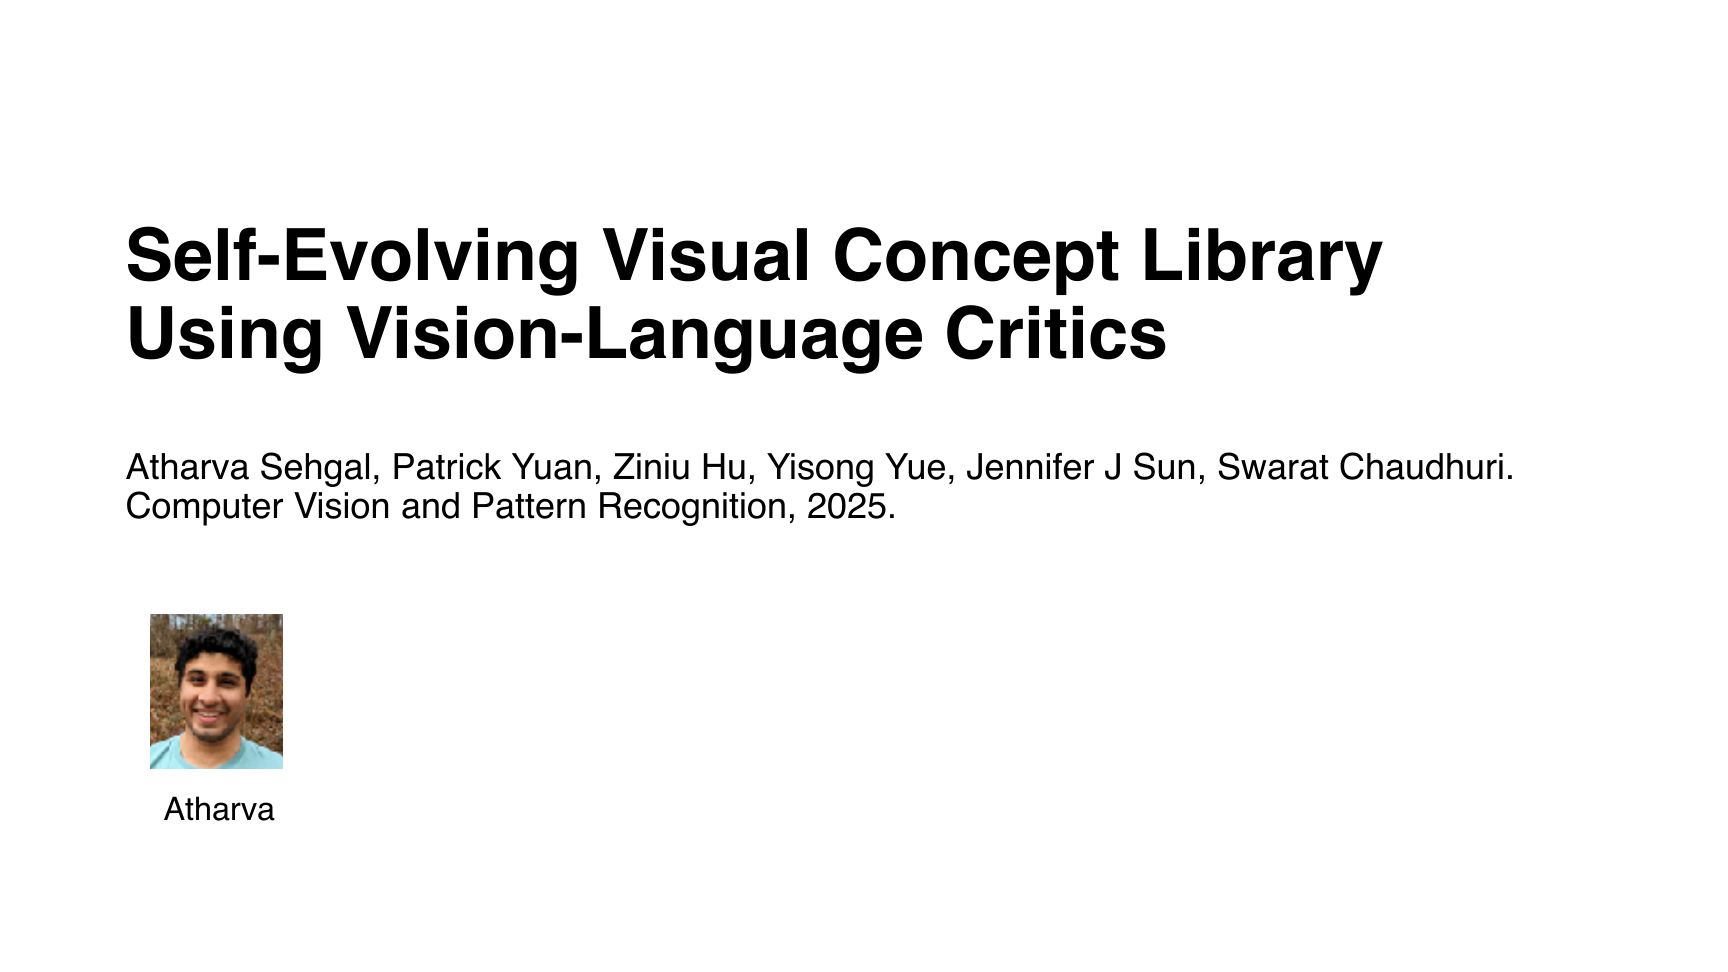
\includegraphics[width=0.80\textwidth]{figures/lec11_fig_012.png}
\caption{visual concept library：用 vision-language critics 进化和评估视觉概念描述。}
\end{figure}

本讲还进一步把 concept discovery 扩展到视觉输入。这里的难点不是再写一个公式，而是学习一组可被 VLM 使用的 visual concept descriptors，然后借助 critic 反馈做 refinement。这为 multimodal agent 提供了一个重要连接点：GUI agent、web agent、OS agent 之所以容易犯错，往往正是因为它们缺少稳定、可组合的视觉概念表示。

\section{开放问题与课程衔接}

\subsection{lecture 给出的 open challenges}

\begin{figure}[H]
\centering
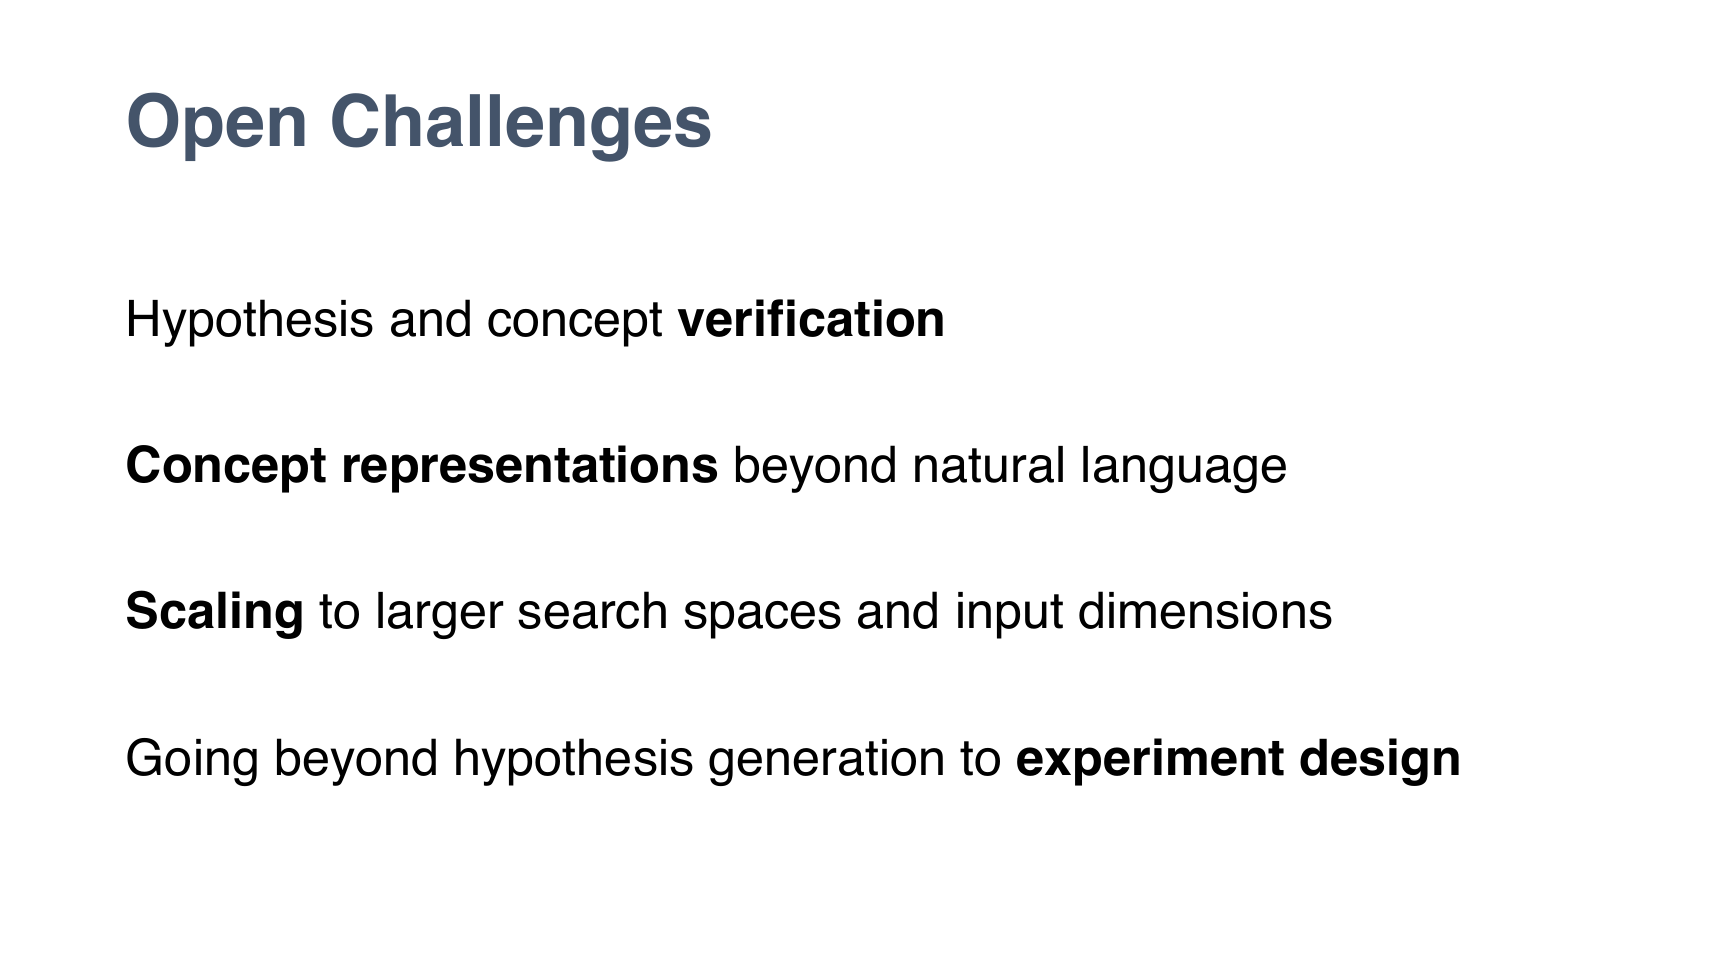
\includegraphics[width=0.82\textwidth]{figures/lec11_fig_013.png}
\caption{lecture 最后一页的 open challenges：验证 hypothesis 与 concepts、扩展表示、扩大搜索空间、推进到 experiment design。}
\end{figure}

slides 的最后总结非常重要。它没有把 abstraction/discovery 说成已经解决的任务，而是明确指出四个开放问题：
\begin{itemize}
\item \textbf{Hypothesis and concept verification}：即便提出了好假设，好概念，如何验证它们仍然困难。
\item \textbf{Concept representations beyond natural language}：自然语言是强大的元表示，但未必是唯一或最佳的概念载体。
\item \textbf{Scaling to larger search spaces and input dimensions}：真实科学任务与视觉任务的搜索空间远大于 lecture 中的 toy setup。
\item \textbf{Going beyond hypothesis generation to experiment design}：真正的 scientific agent 还要能提出该做什么实验，而不仅是拟合已有数据。
\end{itemize}

\subsection{与整门课的联系}

本讲其实把整门课前面的主题收束成一个统一框架。L01--L07 讨论 reasoning、tool use、multimodal action；L08--L10 讨论 formal math、proof search、verification。到这一讲，这些线索开始合流：agent 要能在 discovery 任务里做 search、利用 external feedback、维护记忆和 context、并学会发明更高层的 abstractions。下一讲关于 safe and secure agentic AI，则会把这些能力重新放回安全约束之下：一个会 discovery 的 agent，也必须是可控和可审计的。

\section{本章小结}

本讲最重要的观点是：\textbf{abstraction 不是讲解层面的美化，而是 agent 能否高效 discovery 的结构性条件。} 在数学 discovery 里，它表现为 formal representations、hierarchical reasoning、COPRA 这类 theorem-proving loop；在 scientific discovery 里，它表现为 concept library、symbolic regression、visual concept evolution。二者共享同一个核心模式：利用语言模型把历史经验沉淀成更高层的搜索偏置，并通过外部反馈决定哪些偏置值得保留。

\section{复习题}
\begin{enumerate}
\item 本讲给出的 discovery agent 四个关键能力分别是什么？
\item autoformalization、theorem proving、verification 有什么区别？
\item COPRA 为什么比一次性让 LLM 生成 proof 更稳健？
\item compiler verification 例子说明了 theorem-proving agent 哪些额外职责？
\item LaSR 中 concept library 的主要作用是什么？
\end{enumerate}

\section{深入思考题}
\begin{enumerate}
\item 如果一个 discovery agent 只能提出 hypotheses，但不能验证 hypotheses，它在真实科学场景里会如何失败？
\item concept library 是否可能把搜索过度偏向已有模式，从而抑制真正新颖的发现？
\item 讨论 theorem proving 中的 lemma invention 与 scientific discovery 中的 concept discovery 的相似性和差异。
\end{enumerate}

\section{延伸阅读}
\begin{itemize}
\item An In-Context Learning Agent for Formal Theorem-Proving
\item Symbolic Regression with a Learned Concept Library
\end{itemize}

\end{document}
